\documentclass{standalone}
\usepackage{tikz}
\usepackage{ctex,siunitx}
\usepackage{tkz-euclide}
\usepackage{amsmath}
\usetikzlibrary{patterns, calc}
\usetikzlibrary {decorations.pathmorphing, decorations.pathreplacing, decorations.shapes,}
\begin{document}
\small
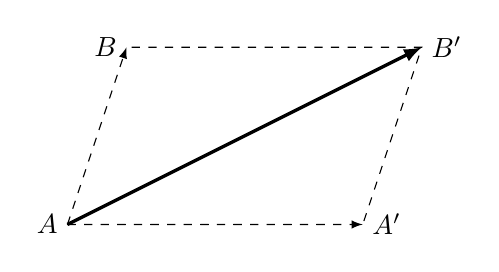
\begin{tikzpicture}[>=latex,scale=1.5]
  \draw [dashed](0,0)node [left]{$A$}--(2.5,0)node [right]{$A'$}
  --(3,1.5)node [right]{$B'$}--(.5,1.5)node [left]{$B$};
  \draw[->, very thick] (0,0)--(3,1.5);
  \draw [dashed,->](0,0)--(2.5,0);
  \draw [dashed,->](0,0)--(.5,1.5);
\end{tikzpicture}
\end{document}